\chapter{Resultados}
\label{chap-results}

Este Capítulo presenta un análisis de los resultados obtenidos a partir de la
ejecución del algoritmo utilizando distintos videos. A lo largo de esta Sección
se refiere al \textit{algoritmo} como a la versión modificada de contornos
activos que fue descripta en el Capítulo \ref{chap-solution}. Las palabras
\textit{aplicación} y \textit{programa} serán utilizadas indistintamente para
referirse al programa que implementa dicho algoritmo, junto con una interfaz de
usuario para el operador. Se refiere a la \textit{implementación} como la parte
del programa que implementa el algoritmo.

En primer lugar, la Sección \ref{sec:aplicacion} describe la aplicación, los
datos que deben ser provistos por el operador, y el funcionamiento de la misma.
La Sección \ref{sec:evaluacion} presenta los resultados obtenidos de la
ejecución del programa y las métricas utilizadas para evaluar la performance de
la implementación. Por último, en la sección \ref{sec:iftrace} se presenta la
comparación con otro método de seguimiento.

\section{Aplicación}
\label{sec:aplicacion}

El programa incorpora una interfaz gráfica utilizada tanto para dar
instrucciones como para recibir información acerca del partido y del
funcionamiento del algoritmo. La misma cuenta con una sección donde se muestra
una lista de los jugadores que están siendo seguidos, una donde se puede
visualizar el video original con un recuadro en cada jugador seguido, un mapa de
calor que muestra las posiciones más frecuentes, y una imagen que permite al
operador evaluar cualitativamente el correcto funcionamiento del algoritmo. Se
puede ver una captura de pantalla de la aplicación en la Figura
\ref{fig:screen1}.

\begin{figure}[H]
  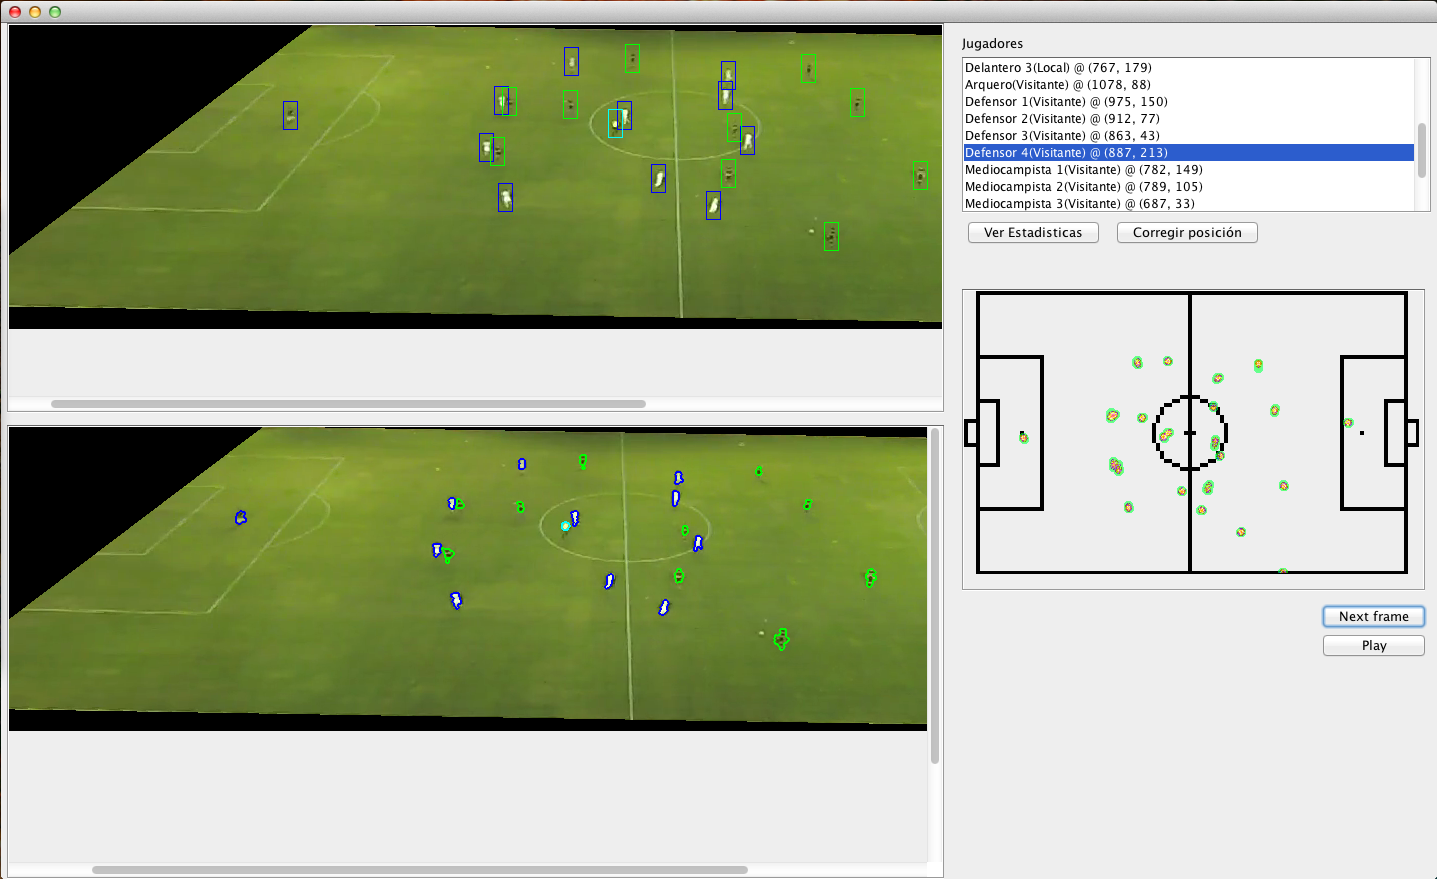
\includegraphics[width=\linewidth]{./images/Screen-Boca.png}
  \captionsetup{justification=centering}
  \caption{Captura de pantalla de la aplicación, mostrando el seguimiento en un video de fútbol.}
  \label{fig:screen1}
\end{figure}

Para comenzar la ejecución del algoritmo, el programa requiere que el operador
identifique la posición de los jugadores en la imagen inicial de la secuencia.
En este paso, también debe agregar información acerca del número de camiseta
que viste, el equipo al cual pertenece y el nombre de cada jugador. Se puede
obtener información de un jugador específico mediante la lista de jugadores
seguidos en la esquina superior derecha. La Figura \ref{fig:screen-jugador}
muestra el detalle con información de un jugador luego de unos segundos de
seguimiento.

\begin{figure}[H]
  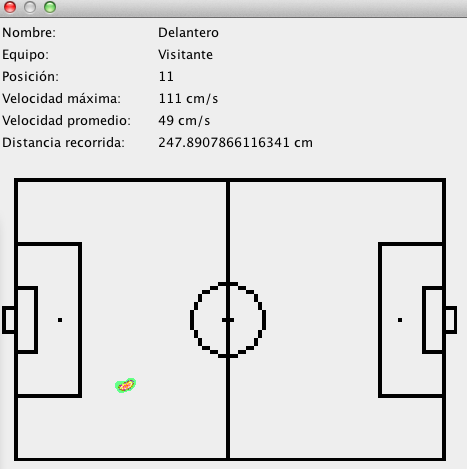
\includegraphics[width=\linewidth]{./images/Screen-Jugador-Stats.png}
  \caption{Captura de pantalla de la aplicación, que muestra información del seguimiento de un jugador.}
  \label{fig:screen-jugador}
\end{figure}

Un paso adicional que debe ejecutar el operador es determinar los puntos a
utilizar para el cálculo de la homografía. Los datos necesarios para ello son
cuatro parejas de puntos, como se explica en la Sección \ref{sec:homography}. De
estas parejas, el primer punto es una coordenada de la imagen en perspectiva y
el otro punto es la coordenada en un plano bidimensional. Con cuatro de estas
relaciones, se puede calcular la matriz que resuelve la homografía para
cualquier otro punto.

Una vez que el programa tiene estos datos, el algoritmo puede comenzar su
ejecución. Existen dos modos: en un modo se puede avanzar un cuadro sólo ante la
indicación del operador (en una mecánica de tipo ``cuadro por cuadro'') y en
otro modo se puede avanzar automáticamente cada vez que se computa un cuadro
(mecánica de tipo ``tiempo real'').

Para cada cuadro, se informa:
\begin{itemize}
\item Posiciones actualizadas de los jugadores
\item Velocidad actual, promedio y máxima de un jugador
\item Mapa de calor del recorrido de cada jugador
\item Mapa de calor del recorrido de todos los jugadores
\end{itemize}

Finalmente, en un archivo se guarda la posición de cada jugador para cada momento.
Y de manera opcional, en cada cuadro se guarda en disco duro una copia del estado
actual del seguimiento para referencia futura.

% TODO: @eordano screenshot del programa aca

\section{Material utilizado}

Se utilizaron principalmente dos videos, uno correspondiente a un partido entre
los equipos argentinos de los clubes Boca Juniors e Independiente; y un segundo
video en el cual se enfrentan los equipos Independiente y San Lorenzo. Se
detalla a continuación las características de las imágenes extraídas de esos
videos.

\begin{itemize}

  \item \textbf{Boca vs. Independiente:} El video cuenta con una resolución de
    \textit{1080p} (1920 píxeles de ancho y 1080 de alto). La cancha se muestra
    en su totalidad, y se puede observar las gradas del lado
    opuesto y cielo por encima de ellas. Luego de descartar esas regiones del
    video, la resolución pasa a ser de 1459 píxeles de ancho por 304 de alto.
    Se puede apreciar en la Figura \ref{fig:boca-figura} un cuadro del video, luego
    de la extracción de las gradas y corrección del efecto de curvatura de la
    lente.

    Los jugadores de Independiente usan remera y shorts de color blanco,
    fácilmente identificables respecto al fondo de color verdoso. El árbitro, de
    amarillo, también contrasta respecto al fondo. Los jugadores de Boca, por
    otro lado, son difíciles de identificar a la distancia y son confundidos con
    el color del césped de la cancha, como se ilustra en la Figura \ref{fig:boca-dificil-1}.

  \item \textbf{Independiente vs. San Lorenzo:} También filmado en resolución de
      \textit{1080p}, las esquinas del campo de juego quedan fuera del campo
      visual. El video fue editado con anterioridad y el alto de un cuadro es
      menor al alto de un video en resolución \textit{1080p}. Luego de descartar
      las gradas, la resolución final del video es de 1920 píxeles de ancho y
      540 de alto. La Figura \ref{fig:independ-figura} muestra un cuadro del
      video procesado.

    Los jugadores de ambos equipos, al utilizar los valores RGB de cada píxel,
    contrastan contra el césped y el algoritmo de contornos activos funciona
    correctamente al analizarlo cualitativamente.

\end{itemize}

\begin{figure}[H]
  \centering
  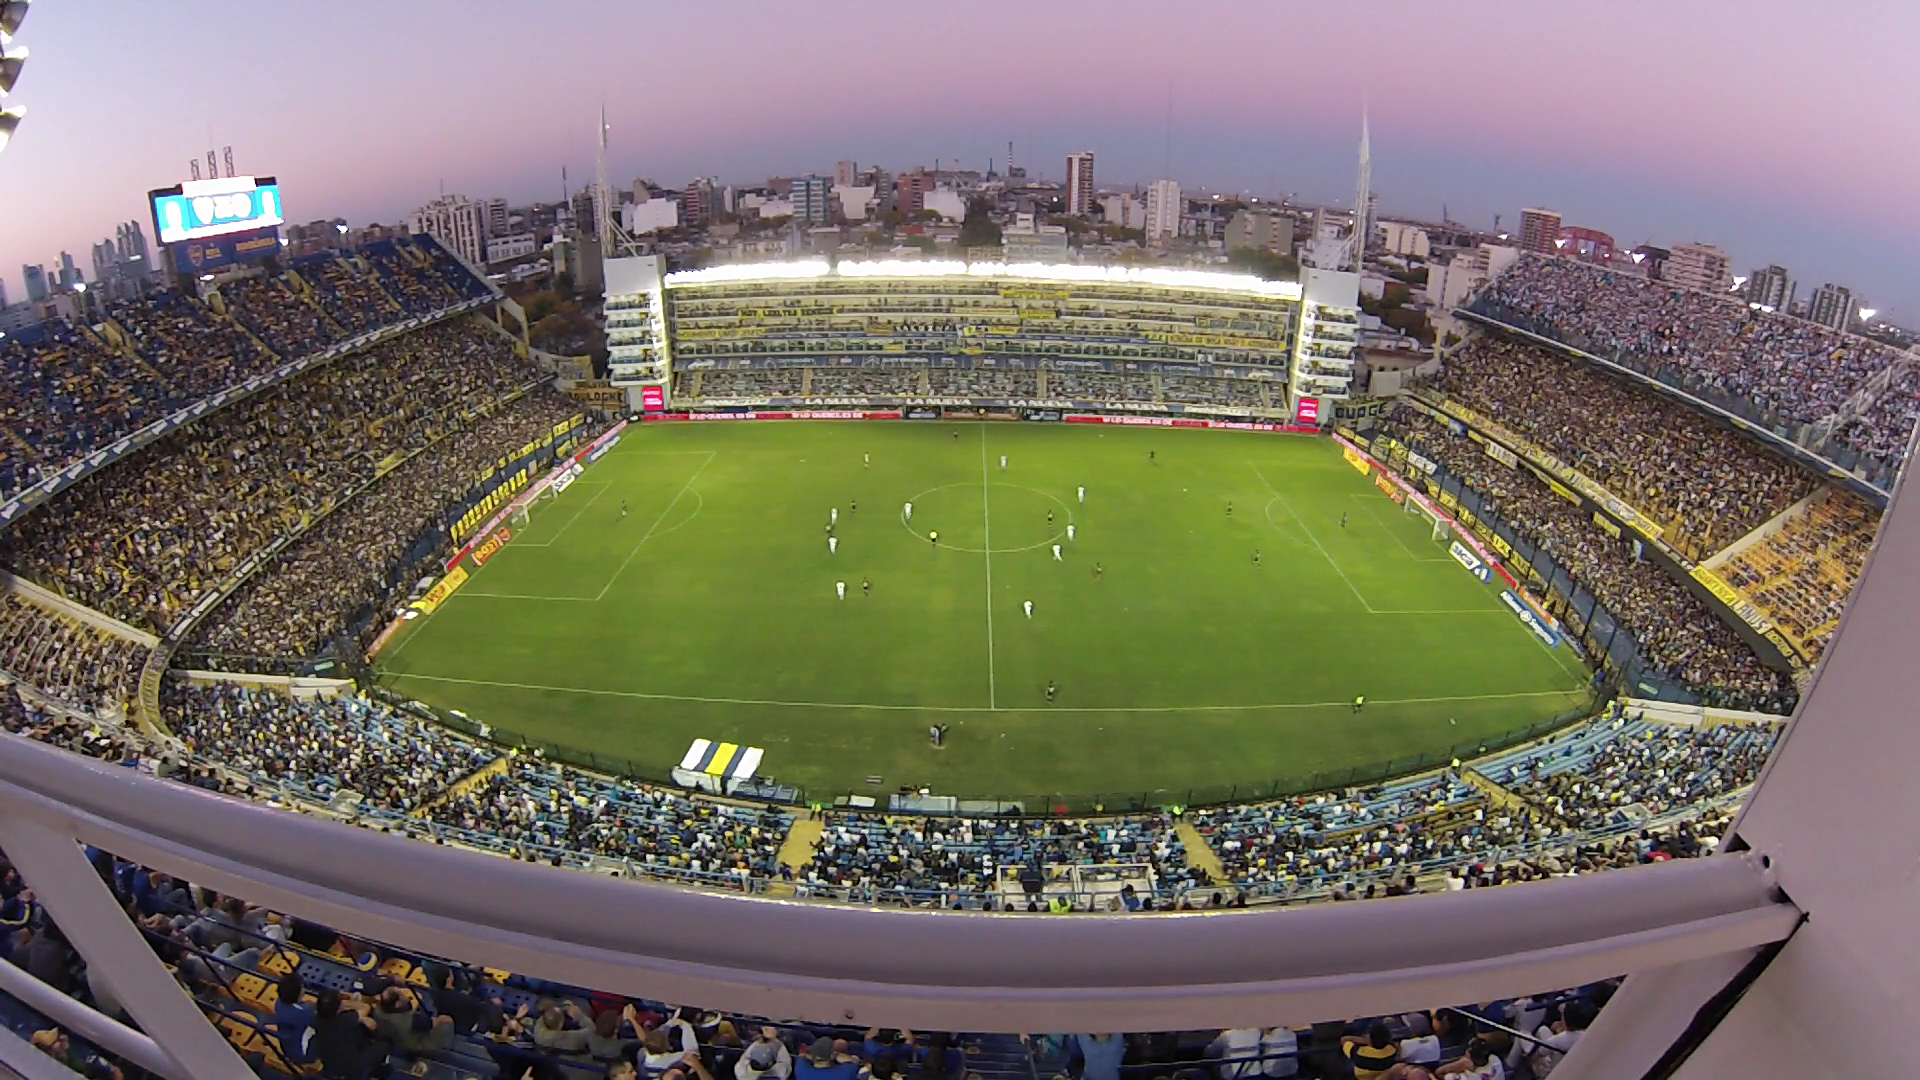
\includegraphics[width=\linewidth]{./images/boca-figura.png}
  \caption{Cuadro del video del partido entre Boca e Independiente.}
  \label{fig:boca-figura}
\end{figure}
\begin{figure}[H]
    \centering
    \captionsetup{justification=centering}
    \begin{minipage}[t]{.5\textwidth}
        \centering
        
\includegraphics[width=.4\linewidth]{./images/boca-dificil1.png}
    \end{minipage}%
    \begin{minipage}[t]{.5\textwidth}
        \centering
        
\includegraphics[width=.4\linewidth]{./images/boca-dificil2.png}
    \end{minipage}
    \caption{Acercamiento a dos jugadores en el video de Boca vs.
             Independiente. De acuerdo a la iluminación, se puede notar que el
             contorno de un jugador puede resultar muy difícil de delimitar.
        \label{fig:boca-dificil-1}}

\end{figure}
\begin{figure}[H]
  \centering
  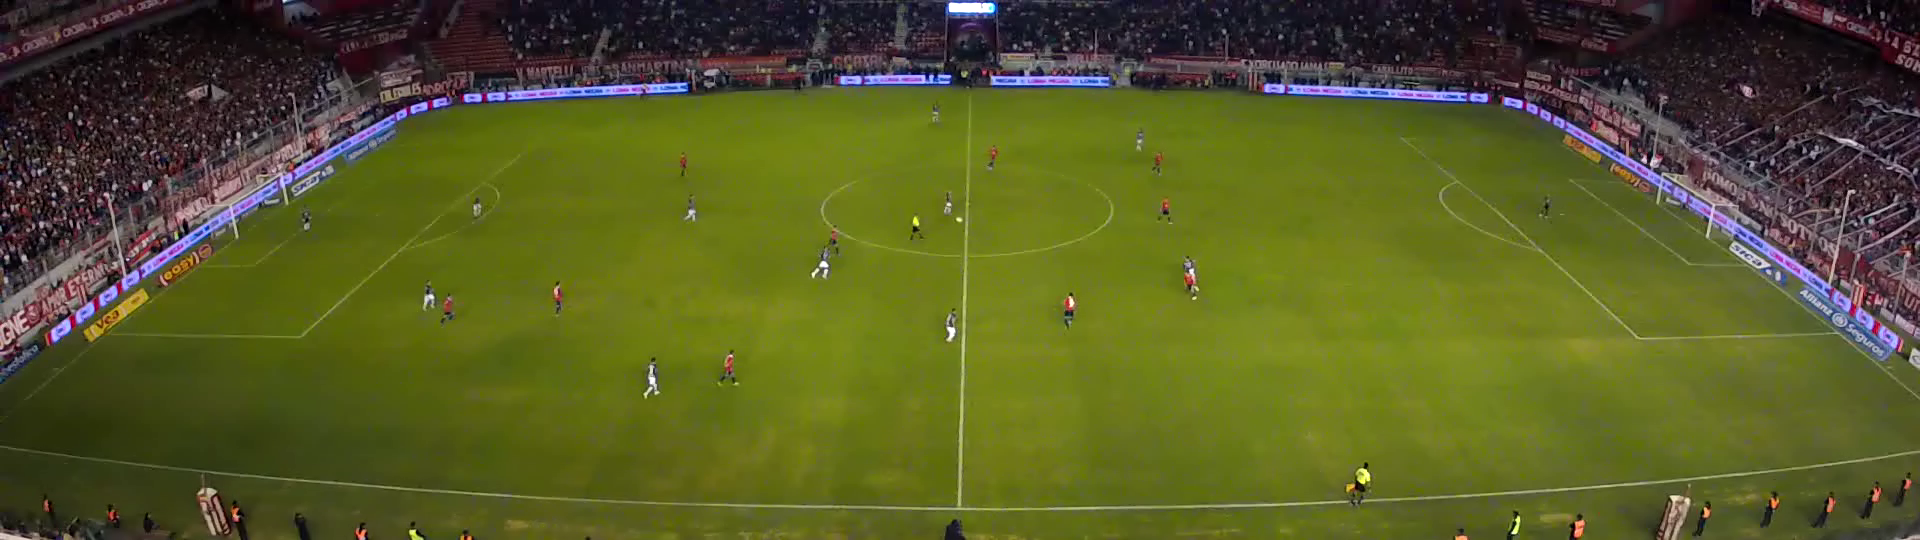
\includegraphics[width=\linewidth]{./images/independ-figura.png}
  \caption{Cuadro del partido en el que Independiente enfrenta a San Lorenzo.}
  \label{fig:independ-figura}
\end{figure}

Además, se tomaron pequeños cortes de tres videos de fútbol televisado, en los
cuales la cámara se encuentra prácticamente estática y se analizó la
correctitud del seguimiento en estos casos, contando con mayor resolución pero
sin poder efectuar exitosamente la eliminación de fondo o la aplicación de una
homografía para determinar las posiciones correctamente, ya que cada cuadro
donde la cámara cambia su orientación, la matriz de la homografía debería ser
recalculada con nuevos datos.

Los videos televisados utilizados pertenecen a tres partidos disputados durante
el año 2014. De la liga \textbf{UEFA}, se tomaron recortes de los partidos
\textbf{Manchester City vs Barcelona FC}, \textbf{Real Madrid vs Borussia
Dortmound}, y de la \textbf{FIFA World Cup} se tomaron fragmentos del partido
de cuartos de final de \textbf{Argentina vs Suiza}.

Del primer video televisado se extrajeron tres escenas en particular. En la
Figura \ref{fig:manchester1} se muestran algunos cuadros de estos fragmentos.
El video cuenta con una resolución de \textit{720p} (1280 píxeles de ancho por
720 píxeles de alto). Los jugadores de Manchester City, con su vestimenta
deportiva de color blanco, son confundidos por sus características con el color
de las líneas de la cancha. En el primer recorte, los jugadores son
correctamente identificados durante los 120 cuadros, exceptuando aquellos que
atraviezan una línea de cancha. Se corrigen correctamente dos oclusiones
parciales entre jugadores. En el segundo fragmento, los jugadores son
correctamente localizados a pesar de la alta velocidad de \textit{panning} de
la cámara. En el tercer video todos los jugadores, al igual que en el primero,
son correctamente localizados durante todo el video exceptuando aquellos que se
intersectan con las líneas marcadas en el césped.

En los otros dos videos se observaron similares características al video de
Manchester City, el seguimiento funciona correctamente bajo la asunción de que
los jugadores no estén ocluyendo una línea en el césped. La Figura
\ref{fig:realmadrid} muestra un cuadro donde se puede apreciar los colores de
la camiseta de ambos equipos en el partido \textbf{Real Madrid vs Borussia
Dortmound} y en la Figura \ref{fig:argentina1} se observa una captura del
partido de \textbf{Argentina vs Suiza}.


\begin{figure}[H]
    \centering
    \captionsetup{justification=centering}
    \begin{minipage}[t]{.45\textwidth}
        \centering
        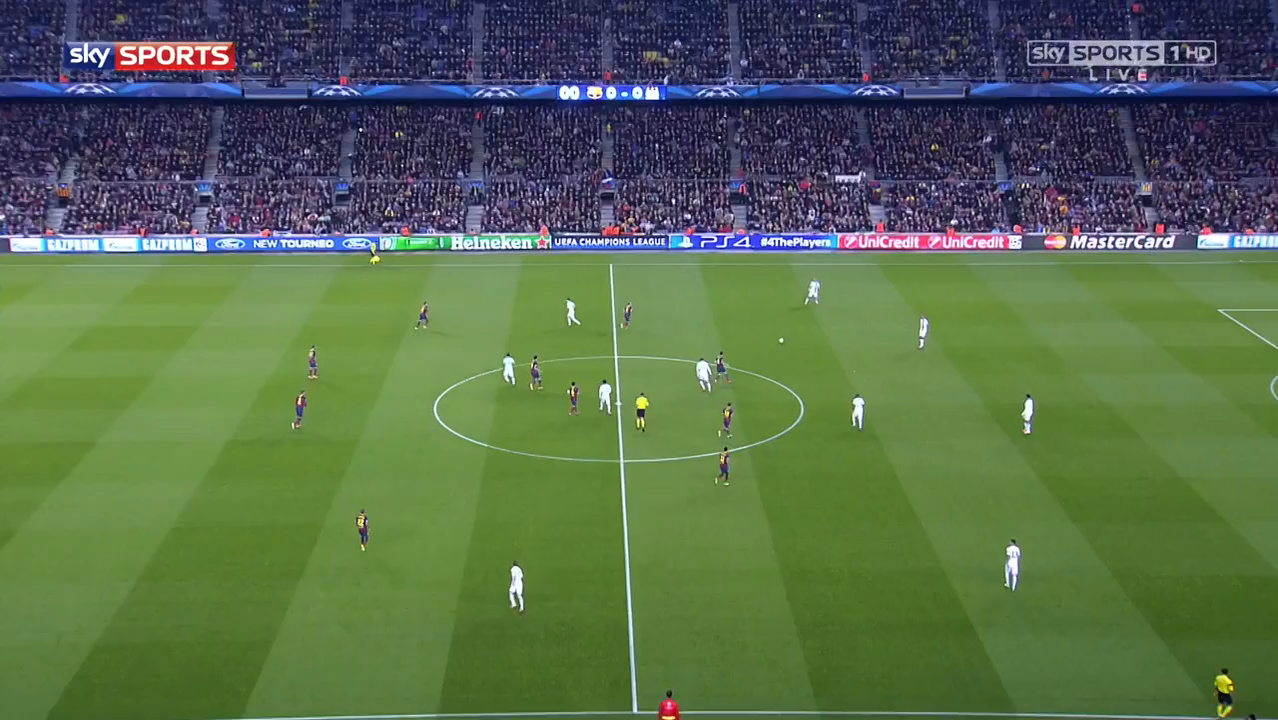
\includegraphics[width=\linewidth]{./images/manchester1.png}
    \end{minipage}%
    \vspace{0.1cm}
    \begin{minipage}[t]{.45\textwidth}
        \centering
        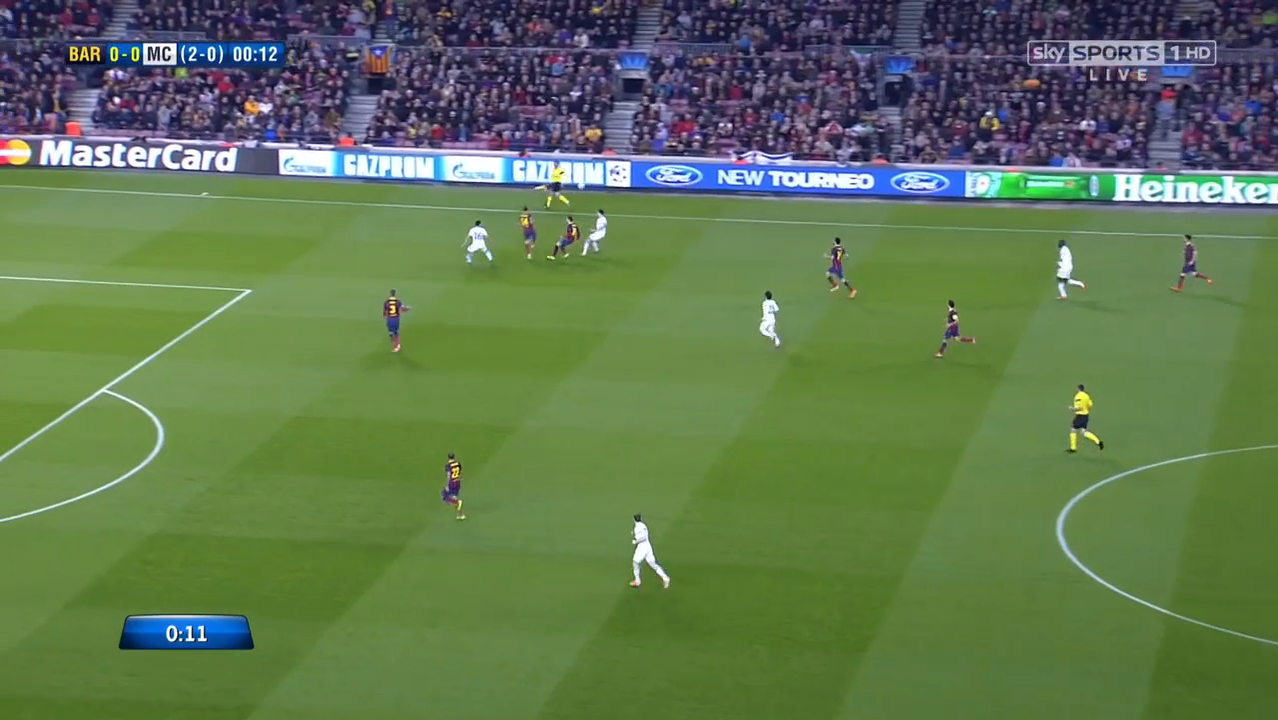
\includegraphics[width=\linewidth]{./images/manchester2.png}
    \end{minipage}
    \caption{Fragmentos del video televizado de un partido entre los equipos Manchester City y Barcelona FC.
        \label{fig:manchester1}}
\end{figure}

\begin{figure}[H]
    \centering
    \captionsetup{justification=centering}
    \begin{minipage}[t]{.45\textwidth}
        \centering
        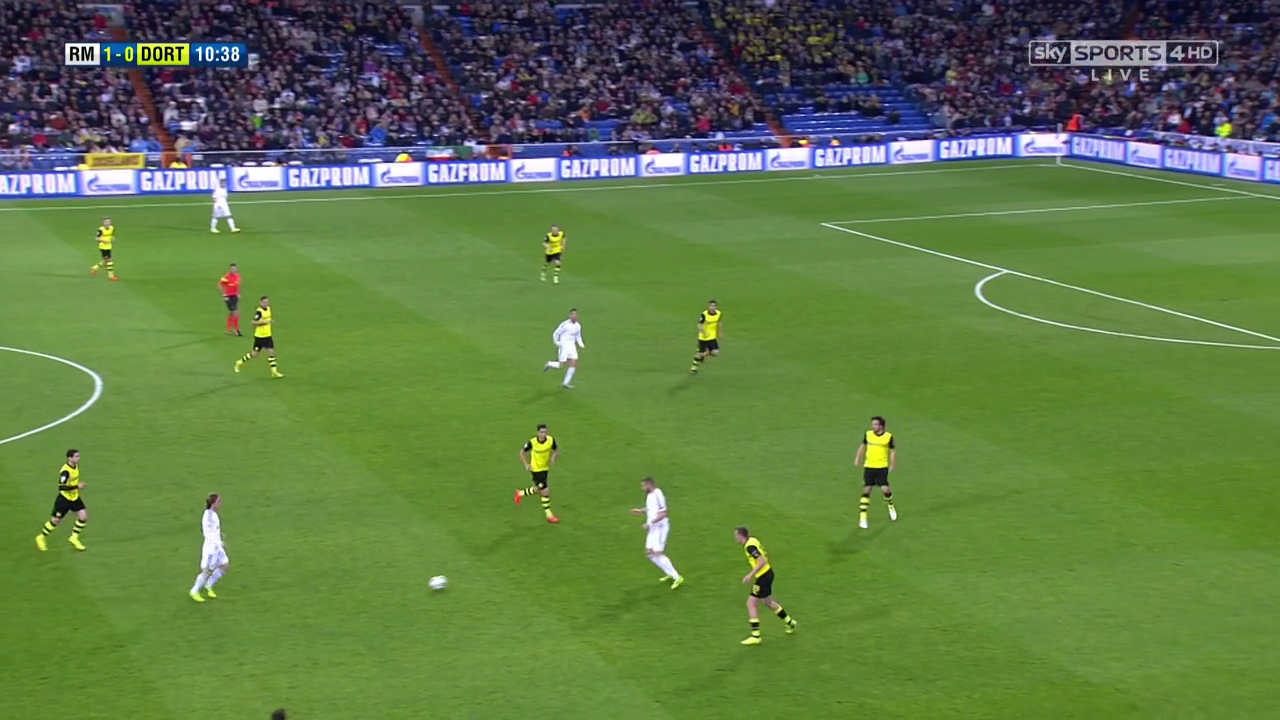
\includegraphics[width=\linewidth]{./images/realmadrid1.png}
        \caption{Real Madrid vs Borussia Dortmound, UEFA Champions League
        \label{fig:realmadrid}}
    \end{minipage}%
    \vspace{0.1cm}
    \begin{minipage}[t]{.45\textwidth}
        \centering
        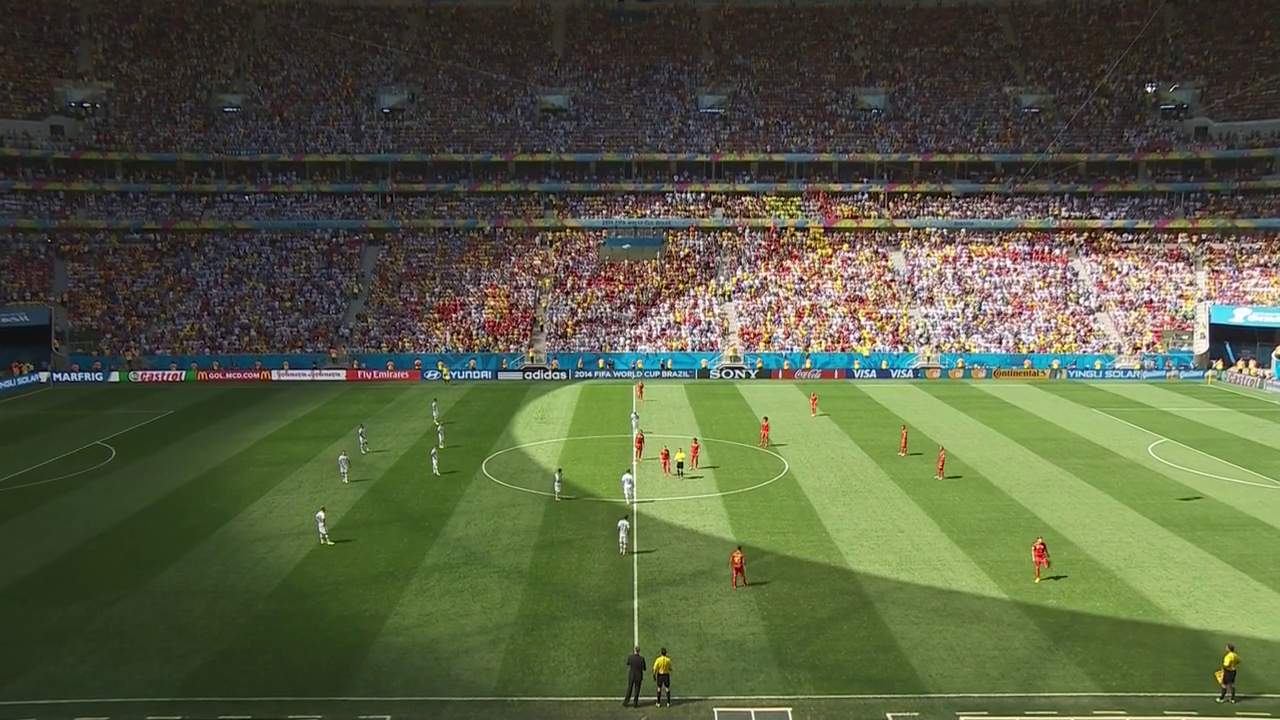
\includegraphics[width=\linewidth]{./images/argentina1.png}
        \caption{Argentina vs Suiza, FIFA World Cup 2014
        \label{fig:argentina1}}
    \end{minipage}
\end{figure}

\section{Evaluación del método}
\label{sec:evaluacion}

La principal evaluación del correcto funcionamiento del algoritmo es llevada a
cabo por el operador de forma cualitativa, como ocurre en otros trabajos
citados en el estado del arte (ver \cite{papers-tanos}). El resultado que
arroja está evaluación es positivo, consiguiéndose seguir correctamente a
todos los jugadores en casi todo momento. Sin embargo, existen algunas
situaciones en las que el algoritmo falla en el seguimiento y no logra
recuperarse por sí mismo, requiriendo una correción manual por parte del
operador para continuar su funcionamiento. Esto se atribuye a la baja calidad
de los videos utilizados como material y a la poca capacidad de procesamiento
en comparación (el poder de procesamiento de una sola computadora limita
algunas operaciones o técnicas).

Las situaciones en que se producen estos errores están bien identificadas
y ocurren porque el algoritmo, en una situación de proximidad entre dos
jugadores, a veces confunde a la sombra del otro jugador con el jugador
al cual se encuentra siguiendo, y comienza a seguir a la sombra, perdiendo
al jugador.

Para evaluar estos inconvenientes se define una métrica que mide exactamente la
cantidad de errores por unidad de tiempo. Esta métrica, resumida como la
cantidad de errores del algoritmo por cada cien cuadros, se intenta minimizar
durante el estudio de las variantes de la aplicación.

La ejecución del algoritmo utilizando el video entre Boca e Independiente
resulta en 7 errores en 766 cuadros, dando aproxidamente 0.91 errores cada cien
cuadros, lo que significa un poco menos de un error cada 4 segundos.

En el video del partido entre Independiente y San Lorenzo el algoritmo incurre
en 6 errores en 213 cuadros, dando 2.81 errores cada cien cuadros. Es decir,
algo menos de 3 errores cada 4 segundos.

Otro aspecto importante a la hora de evaluar la solución propuesta es su
velocidad, medida en el tiempo de ejecución que requiere para llevar a cabo su
trabajo. Para medir esto se define la métrica del tiempo que le toma al
algoritmo procesar un solo cuadro, o, lo que es lo mismo, la cantidad de
cuadros procesados por segundo. El objetivo es minimizar esta métrica
intentando acercarse lo más posible a los $24$ cuadros por segundo (equivalente
a $42$ milisegundos por cuadro), la velocidad de los videos utilizados.

\section{Comparación con IFTrace}
\label{sec:iftrace}

El algoritmo de seguimiento IFTrace, propuesto por \citeauthor*{IFTrace}, es un
algoritmo robusto que soporta cambios de iluminación y forma, oclusiones y se
centra en hallar características representativas de la textura de los objetos a
seguir. Es capaz de recuperarse de errores menores y permite el seguimiento de
múltiples objetos a la vez.

Un algoritmo de este tipo podría proporcionar una solución al problema. Para
comprobarlo, se llevaron a cabo algunas pruebas utilizando un video sintético
creado para este fin, y un video real de un partido de fútbol. En la Figura
\ref{fig:screen1} de la sección anterior se observa un video real. La figura
\ref{fig:sample-happy-occluded} muestra el primer cuadro del video sintético. Pueden
apreciarse a simple vista las marcadas diferencias entre ambos videos, como por
ejemplo la resolución de la imagen y el tamaño y la complejidad de los objetos
de interés.

\begin{figure}[H]
    \centering
    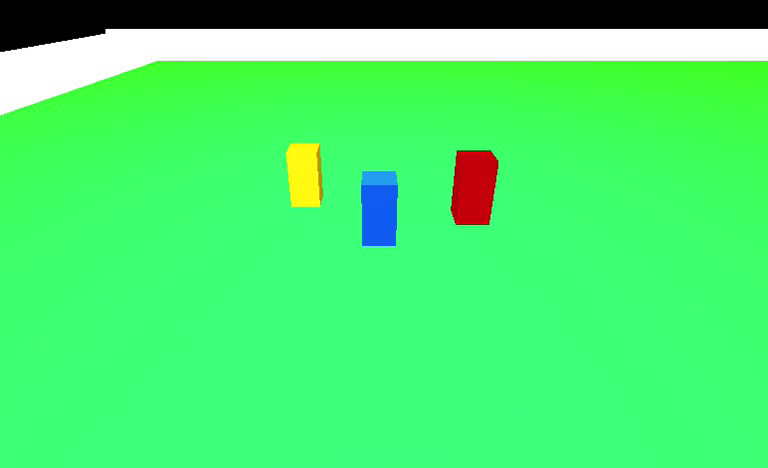
\includegraphics[width=\linewidth]{./images/sample_happy_occluded.png}
    \caption{Muestra de un cuadro del video sintético de prueba.}
    \label{fig:sample-happy-occluded}
\end{figure}

Como se puede ver en la Figura \ref{fig:happy-occluded-iftrace}, IFTrace logra
un correcto seguimiento de múltiples objetos en el video sintético. También
puede observarse, en la Figura \ref{fig:boca-iftrace}, como sigue correctamente
a un jugador en el video real. Sin embargo, el seguimiento sólo es exitoso
durante unos pocos cuadros, ya que, en el cuadro 17, el algoritmo cae en un
error del cual sólo una corrección manual puede sacarlo. Este tipo de corrección
semi-supervisada no está contemplada en el algoritmo de IFTrace.

\begin{figure}[H]
    \centering
    \begin{minipage}[t]{.25\textwidth}
      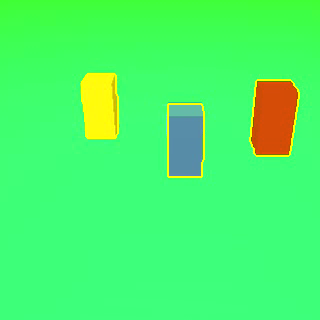
\includegraphics[width=1.4in]{./images/cropped_happy_occluded_00001.png}
      \centering
      \footnotesize
      \textbf{(a)} Cuadro 1
    \end{minipage}
    \hspace{-0.3cm}
    \begin{minipage}[t]{.25\textwidth}
      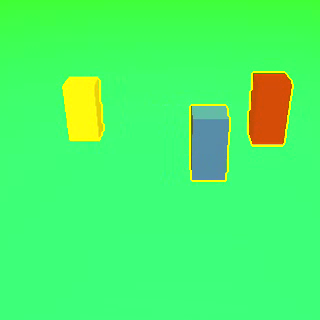
\includegraphics[width=1.4in]{./images/cropped_happy_occluded_00005.png}
      \centering
      \footnotesize
      \textbf{(b)} Cuadro 5
    \end{minipage}
    \hspace{-0.3cm}
    \begin{minipage}[t]{.25\textwidth}
      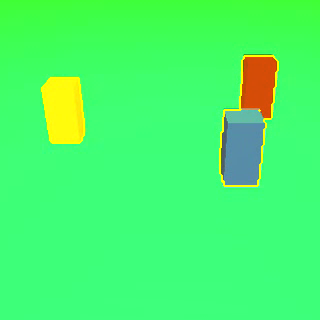
\includegraphics[width=1.4in]{./images/cropped_happy_occluded_00008.png}
      \centering
      \footnotesize
      \textbf{(c)} Cuadro 8
    \end{minipage}
    \hspace{-0.3cm}
    \begin{minipage}[t]{.25\textwidth}
      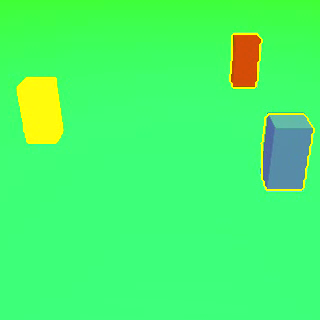
\includegraphics[width=1.4in]{./images/cropped_happy_occluded_00012.png}
      \centering
      \footnotesize
      \textbf{(d)} Cuadro 12
    \end{minipage}
    %% NASTY hack to make refernce work with figures and subfigures, put \label inside \caption env, little bird told me
    \caption{IFTrace funcionando en una secuencia de cuadros de video sintético.
    \label{fig:happy-occluded-iftrace}
    }
\end{figure}

\begin{figure}[H]
    \centering
    \begin{minipage}[t]{.25\textwidth}
      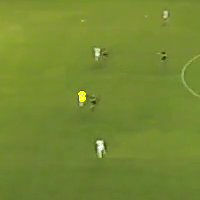
\includegraphics[width=1.4in]{./images/cropped_boca_00009.png}
      \centering
      \footnotesize
      \textbf{(a)} Cuadro 9
    \end{minipage}
    \hspace{-0.3cm}
    \begin{minipage}[t]{.25\textwidth}
      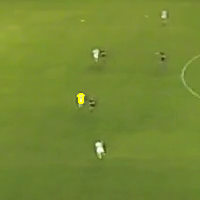
\includegraphics[width=1.4in]{./images/cropped_boca_00012.png}
      \centering
      \footnotesize
      \textbf{(b)} Cuadro 12
    \end{minipage}
    \hspace{-0.3cm}
    \begin{minipage}[t]{.25\textwidth}
      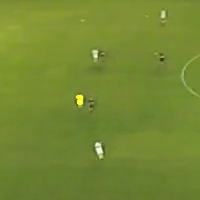
\includegraphics[width=1.4in]{./images/cropped_boca_00014.png}
      \centering
      \footnotesize
      \textbf{(c)} Cuadro 14
    \end{minipage}
    \hspace{-0.3cm}
    \begin{minipage}[t]{.25\textwidth}
      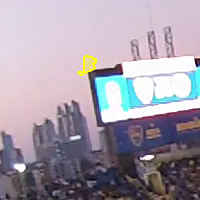
\includegraphics[width=1.4in]{./images/cropped_boca_00017.png}
      \centering
      \footnotesize
      \textbf{(d)} Cuadro 17
    \end{minipage}
    %% NASTY hack to make refernce work with figures and subfigures, put \label inside \caption env, little bird told me
    \caption{Seguimiento de un jugador en un video real utilizando IFTrace.
    \label{fig:boca-iftrace}
    }
\end{figure}

\begin{figure}[H]
    \centering
    \begin{minipage}[t]{.25\textwidth}
      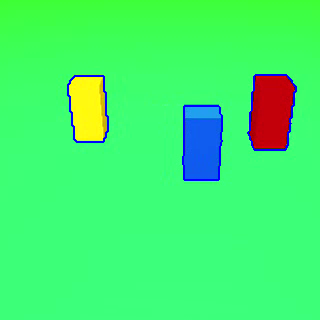
\includegraphics[width=1.4in]{./images/cropped_processing2.png}
      \centering
      \footnotesize
      \textbf{(a)} Cuadro 1
    \end{minipage}
    \hspace{-0.3cm}
    \begin{minipage}[t]{.25\textwidth}
      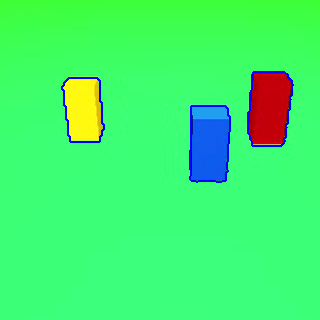
\includegraphics[width=1.4in]{./images/cropped_processing5.png}
      \centering
      \footnotesize
      \textbf{(b)} Cuadro 5
    \end{minipage}
    \hspace{-0.3cm}
    \begin{minipage}[t]{.25\textwidth}
      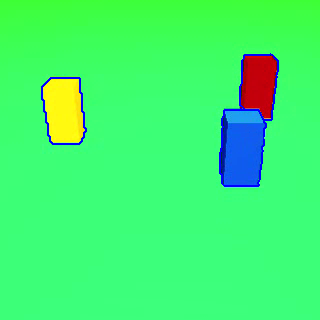
\includegraphics[width=1.4in]{./images/cropped_processing14.png}
      \centering
      \footnotesize
      \textbf{(c)} Cuadro 8
    \end{minipage}
    \hspace{-0.3cm}
    \begin{minipage}[t]{.25\textwidth}
      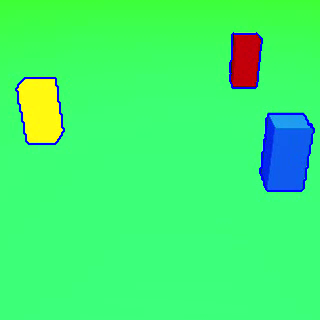
\includegraphics[width=1.4in]{./images/cropped_processing25.png}
      \centering
      \footnotesize
      \textbf{(d)} Cuadro 12
    \end{minipage}
    %% NASTY hack to make refernce work with figures and subfigures, put \label inside \caption env, little bird told me
    \caption{El algoritmo de contornos activos modificado en funcionamiento en un video sintético.
    \label{fig:happy-occluded-activeContour}
    }
\end{figure}

\begin{figure}[H]
    \centering
    \begin{minipage}[t]{.25\textwidth}
      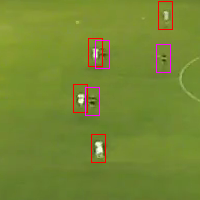
\includegraphics[width=1.4in]{./images/cropped_rendered002.png}
      \centering
      \footnotesize
      \textbf{(a)} Cuadro 2
    \end{minipage}
    \hspace{-0.3cm}
    \begin{minipage}[t]{.25\textwidth}
      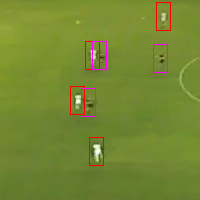
\includegraphics[width=1.4in]{./images/cropped_rendered007.png}
      \centering
      \footnotesize
      \textbf{(b)} Cuadro 12
    \end{minipage}
    \hspace{-0.3cm}
    \begin{minipage}[t]{.25\textwidth}
      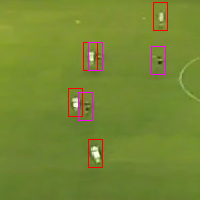
\includegraphics[width=1.4in]{./images/cropped_rendered012.png}
      \centering
      \footnotesize
      \textbf{(c)} Cuadro 14
    \end{minipage}
    \hspace{-0.3cm}
    \begin{minipage}[t]{.25\textwidth}
      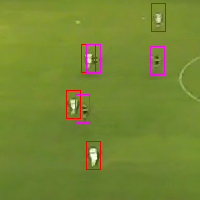
\includegraphics[width=1.4in]{./images/cropped_rendered017.png}
      \centering
      \footnotesize
      \textbf{(d)} Cuadro 17
    \end{minipage}
    %% NASTY hack to make refernce work with figures and subfigures, put \label inside \caption env, little bird told me
    \caption{Seguimiento de los jugadores en un video real mediante el algoritmo de contornos activos modificado.
    \label{fig:boca-activeContour}
    }
\end{figure}

Como se puede observar en la Figura \ref{fig:happy-occluded-activeContour}, el
algoritmo propuesto en este trabajo logra seguir con éxito a los objetos de
interés en el video sintético. Además, también se obtiene un resultado positivo
en el video real en la situación en que IFTrace pierde al jugador, como puede
observarse en la Figura \ref{fig:boca-activeContour}.

\subsection{Evaluación de Comportamiento}

Otro punto importante de comparación entre los dos algoritmos es su tiempo de
ejecución, es decir el tiempo que tarda en llevar a cabo su trabajo.  De
acuerdo a las mediciones realizadas con un video real de un partido de fútbol,
siguiendo a un solo jugador, el tiempo promedio que tarda IFTrace por cuadro es
6.962 segundos, mientras que el algoritmo implementado tiene un tiempo promedio
de 0.712 segundos. Se puede observar que se encuentra un orden magnitud por
debajo de IFTrace, incluso antes de realizar optimizaciones.
%% 6.9628571428571435 si quieren los decimales

Cabe destacar que ambos algoritmos podrían verse beneficiados de ciertas
optimizaciones, como ser por ejemplo la programación en GPU y la reducción de
operaciones de \textit{Input/Output} al almacenamiento secundario (disco duro).

